Entre las fuerzas actúan sobre la gota de aceite se encuentran: la fuerza
gravitacional $\vec{F}_g$, la fuerza de empuje o flotabilidad descrita
por el principio de Arquímedes $\vec{F}_b$ y la fuerza de fricción generada
por el aire $\vec{F}_d$, que se modela a través de la ley de Stokes.

\begin{figure}[htbp!]
    \centering
    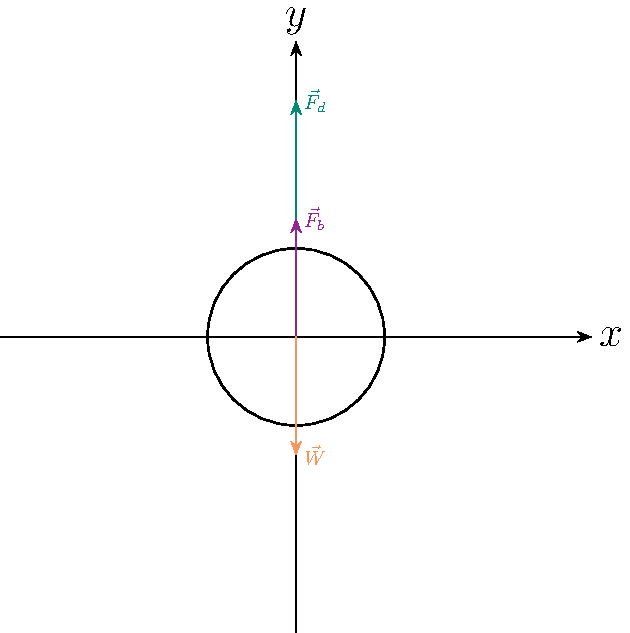
\includegraphics[width=0.8\linewidth]{./images/free-body-diagram-falling.pdf}
    \caption{Diagrama de cuerpo libre de la gota de aceite en descenso.}
    \label{fig:fbd-falling-drop}
\end{figure}

Inicialmente, la gota es acelerada hacia la Tierra, pero rápidamente
alcanza una velocidad terminal, lo que indica un estado de equilibrio de fuerzas.
En este punto, como se muestra en la \cref{fig:fbd-falling-drop}, la suma de
las fuerzas que actúan sobre la gota es cero.
\begin{equation}\label{eq:equilibrium-1}
    \vec{F}_d + \vec{F}_b + \vec{F}_g = 0
\end{equation}

Las expresiones de las fuerzas gravitacional, de flotación y de fricción se
muestran en las \cref{eq:grav,eq:bouyant,eq:drag} respectivamente, donde
\( V_{ac} \) representa el volumen de la gota de aceite y
\( mu = \qty{1.85e-5}{kgm^{-1}s^{-1}} \) el coeficiente de viscosidad del aire.
\begin{align}
    \vec{F}_g &= m\vec{g} \label{eq:grav} \\
    \vec{F}_b &= -\rho_a \vec{g}V_{ac} \label{eq:bouyant} \\
    \vec{F}_d &= -6\pi r\mu \vec{v}_c \label{eq:drag}
\end{align}

Tomando en cuenta solo las magnitudes de estas fuerzas y sustituyendo en la
ecuación de equilibrio (\cref{eq:equilibrium-1}) se obtiene la \cref{eq:system-1}
donde las incógnitas son la masa \(m\), el volumen \(V_{ac}\) y el radio \(r\)
de la gota.
Debido a la dificultad de medir directamente la masa de la gota, el volumen y la
masa se expresan en términos de \(r\) y de la densidad del aceite \(\rho_{ac}\),
como se muestra en las \cref{eq:mass,eq:volume}.
\begin{equation}\label{eq:system-1}
    6\pi r\mu v_c = mg - \rho_a g V_{ac}
\end{equation}
\begin{align}
    V_{ac} = \frac{4}{3}\pi r^3 \label{eq:volume} \\
    m = \frac{4}{3}\pi r^3\rho_{ac} \label{eq:mass}
\end{align}

Al remplazar, se despeja \( r \) obteniendo la relación mostrada en la
\cref{eq:radius}.
\begin{equation}\label{eq:radius}
    r = \sqrt{\frac{9\mu v_c}{2g(\rho_{ac}-\rho_a)}}
\end{equation}

En el segundo escenario, cuando se aplica una campo eléctrico, la gota comienza
a ascender.
Al alcanzar a una velocidad terminal $v_a$ las fuerzas sobre la gota se
equilibran,incluyendo la fuerza eléctrica \(\vec{F}_e\), como se ilustra en la
\cref{fig:fbd-ascending-drop}.
\begin{equation}
    \vec{F}_E + \vec{F}_e + \vec{F}_g + \vec{F}_d = 0
\end{equation}

\begin{figure}[htbp!]
    \centering
    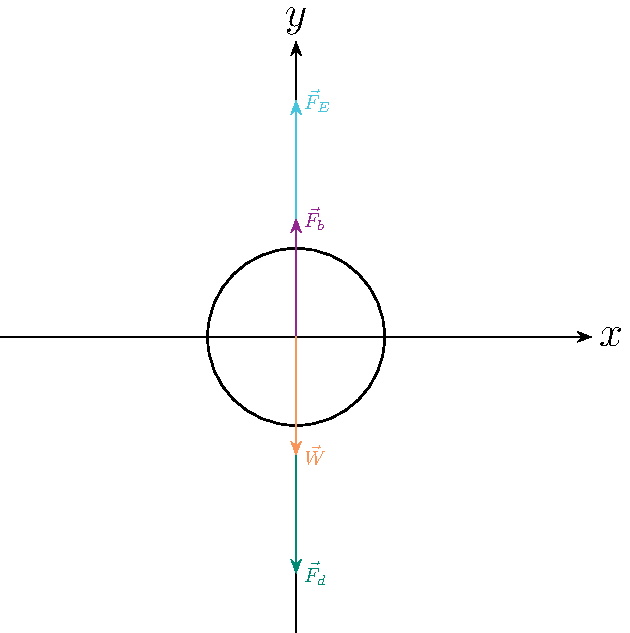
\includegraphics[width=0.8\linewidth]{./images/free-body-diagram-ascending.pdf}
    \caption{Diagrama de cuerpo libre de la gota de aceite en ascenso}
    \label{fig:fbd-ascending-drop}
\end{figure}

Utilizando las magnitudes de las fuerzas previamente conocidas y remplazando
\(F_e=qE \), donde $E$ es el campo eléctrico, se obtiene la segunda ecuación de
equilibrio (\cref{eq:system-2}).
\begin{equation}\label{eq:system-2}
    qE = 6\pi r\mu v_a + \frac{4}{3}\pi r^3(\rho_{ac}-\rho_a)
\end{equation}

Dado que previamente se ha determinado el valor de \(r\), y sabiendo que el campo
eléctrico en un capcacitor se define por \( E = U / d \), donde $U$ es la
diferencia de potencial aplicada y $d$ es la separación entre placas, se obtiene
la \cref{eq:charge} para la carga \(q\) de la gota en términos de las magnitudes
conocidas.
\begin{equation}\label{eq:charge}
    q = \frac{6\pi \mu d}{U}\sqrt{\frac{9\mu v_c}{2g(\rho_{ac}-\rho_a)}}(v_a-v_c)
\end{equation}

Finalmente, dado que la carga eléctrica está cuantizada \cite{}, es decir,
debe ser un múltiplo entero de la carga elemental \(e^{-}\), se cumple la
relación de la \cref{eq:quantized}.
\begin{equation}\label{eq:quantized}
    q=ne^-
\end{equation}

Realizando un número suficiente de mediciones de \(q\) y aplicando el algoritmo
euclídeo para determinar el mínimo común divisor \cite{}, es posible obtener el
valor de \(e^{-}\), que corresponde a la carga elemental de un electrón.
